%% 
%% Copyright 2007, 2008, 2009 Elsevier Ltd
%% 
%% This file is part of the 'Elsarticle Bundle'.
%% ---------------------------------------------
%% 
%% It may be distributed under the conditions of the LaTeX Project Public
%% License, either version 1.2 of this license or (at your option) any
%% later version.  The latest version of this license is in
%%    http://www.latex-project.org/lppl.txt
%% and version 1.2 or later is part of all distributions of LaTeX
%% version 1999/12/01 or later.
%% 
%% The list of all files belonging to the 'Elsarticle Bundle' is
%% given in the file `manifest.txt'.
%% 

%% Template article for Elsevier's document class `elsarticle'
%% with numbered style bibliographic references
%% SP 2008/03/01

\documentclass[preprint,12pt, a4paper]{elsarticle}

%% Use the option review to obtain double line spacing
%% \documentclass[authoryear,preprint,review,12pt]{elsarticle}

%% For including figures, graphicx.sty has been loaded in
%% elsarticle.cls. If you prefer to use the old commands
%% please give \usepackage{epsfig}

%% The amssymb package provides various useful mathematical symbols
\usepackage{amssymb}
%% The amsthm package provides extended theorem environments
\usepackage{amsthm}
\usepackage{mathtools}
%% The lineno packages adds line numbers. Start line numbering with
%% \begin{linenumbers}, end it with \end{linenumbers}. Or switch it on
%% for the whole article with \linenumbers.
\usepackage{lineno}

\usepackage{float}

\usepackage{todonotes} 
\usepackage{url}

\restylefloat{table}

\newcommand{\eg}{{\emph{e.g.\/}}}
\newcommand{\ie}{{\emph{i.e.\/}}}
\newcommand{\ket}[1]{\ensuremath{|#1\rangle}}
\newcommand{\bra}[1]{\ensuremath{\langle#1|}}
\newcommand{\ketbra}[2]{\ensuremath{\ket{#1}\bra{#2}}}
\newcommand{\proj}[1]{\ensuremath{\ketbra{#1}{#1}}}
\newcommand{\braket}[2]{\ensuremath{\langle{#1}|{#2}\rangle}}
\newcommand{\floor}[1]{\ensuremath{\lfloor #1 \rfloor}}
\newcommand{\complexity}[1]{\ensuremath{\mathbf{#1}}}
\newcommand{\new}[1]{ \textcolor{red}{#1} }
\newcommand{\1}{{\rm 1\hspace{-0.9mm}l}}
\newcommand{\Id}{{\rm 1\hspace{-0.9mm}l}}
\newcommand{\connected}{\sim}
\newcommand{\SPAN}{\mathrm{span}}
\newcommand{\Lrm}{\ensuremath{\mathrm{L}}}
\newcommand{\Urm}{\ensuremath{\mathrm{U}}}
\newcommand{\ee}{\ensuremath{\mathrm{e}}}
\newcommand{\dd}{\ensuremath{\mathrm{d}}}
\newcommand{\ii}{\ensuremath{\mathrm{i}}}
\newcommand{\EE}{\mathcal{E}}
\newcommand{\XX}{\mathcal{X}}
\newcommand{\MM}{\mathcal{M}}
\newcommand{\NN}{\mathcal{N}}
\newcommand{\DD}{\mathcal{D}}
\newcommand{\TT}{\mathcal{T}}
\newcommand{\PP}{\mathcal{P}}
\newcommand{\QQ}{\mathcal{Q}}
\renewcommand{\SS}{\mathcal{S}}
\newcommand{\UU}{\mathcal{U}}
\newcommand{\HH}{\mathcal{H}}
\newcommand{\DU}{\mathcal{DU}}
\newcommand{\NOT}{\sigma_x}
\newcommand{\idop}[1][\XX]{\ensuremath{\1_{#1}}}
\newcommand{\diaguni}{\ensuremath{\mathcal{DU}}}
\newcommand{\diag}{\mathrm{diag}}
\newcommand{\tr}{\mathrm{tr}}
%\DeclareMathOperator{\diag}{diag}
%\DeclareMathOperator{\diag}{diag}
\journal{SoftwareX}


\usepackage{amsmath}
\newtheorem{theorem}{Theorem}
\newtheorem{proposition}{Proposition}
\newtheorem{remark}{Remark}
\newtheorem{scheme}{Scheme}
\newtheorem{lemma}{Lemma}

\begin{document}



\subsubsection{Motivation}

Suppose we have access to a device performing one of the predefined von Neumann
measurements\footnote{In PyQBench, we restrict ourselves to discriminating von Neumann measurements.
This is because, unlike other measurement types, they can be implemented on actual hardware.
},  $\PP$ or $\QQ$. While the $\PP$ and $\QQ$ are known, it is not known which of them is
performed when the device executes. Based on the measurement outcome, you have to guess which
measurement was performed (but you can perform arbitrary unitary operations before and after the
measurement). What is the highest probability of making a correct guess? And what do you have to do
to achieve it? And, most importantly, why would we want to do this?

Suppose that you know a strategy that, for an ideal device, would yield a probability
$p_{\text{succ}}$ of successfully discriminating between two measurements. Will the probability be
the same on an actual physical device? For current, Noisy Intermediate Scale Quantum devices
(NISQs), the answer is: certainly not. However, the error rate that you make when guessing can be
used as a benchmarking metric. PyQBench helps you in organizing such discrimination experiments for
a single qubit system\footnote{As we will soon see, the optimal discrimination strategy requires
the usage of an additional auxiliary qubit.}, executing them on real hardware or simulators, and
computing discrimination probabilities based on the measured bitstrings.

\subsubsection{Discrimination scheme}

Without loss of generality, we consider discrimination between a measurement in the computational
Z-basis ($\PP_\Id$), and an alternative measurement performed in the basis $U$
($\PP_U$)\footnote{Explaining why we can consider only Z-basis and alternative measurement is beyond
the scope of this technical documentation. See \cite{puchala2018strategies} if you are interested in
the explanation.}. In PyQBench, we operate only on two-level systems, but the discrimination scheme,
described in detail in \cite{puchala2018strategies}, makes no assumptions about the dimensionality.

In general, the discrimination scheme, presented in Fig.\ref{fig:theoretical_scheme}, requires a
second system of the same dimensionality as the measured one. First, the joint system is prepared in
some state $\ket{\psi_0}$. Then, the unknown measurement is performed on the first part of the
system. Based on its outcome $i$, another measurement $\mathcal{P}_{V_i}$ is performed to obtain an
outcome $j$. Finally, if $j=0$ we guess that the performed measurement is $\mathcal{P}_U$, otherwise
we guess that it was $\mathcal{P}_\Id$.

\begin{figure}[h!]
	\centering
	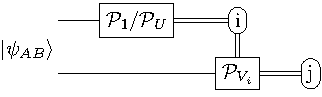
\includegraphics[scale=1.7]{pics/theoretical_scheme}
	\caption{Theoretical  scheme of discrimination  between von Neumann measurements $\PP_{U}$ and $\PP_\Id$. }
	\label{fig:theoretical_scheme}
\end{figure}

\subsubsection{Quantum architecture's limits and practical solutions}


Let us take a closer look at the setup for distinguishing von Neumann 
measurements (see Fig.~\ref{fig:theoretical_scheme}). One of the components of 
this scheme is to perform a conditional  measurement. 
However, current NISQ devices do not allow for performing conditional 
 measurements.

We  will present two possible methods providing a clever way to cross this 
obstacle. These will be two schemes of practical realization. 
The first method consists in using postselection while the second method 
consists in applying a controlled unitary. These methods are described below. 

\begin{scheme}(Postselection)



%\begin{figure}[h!]
%	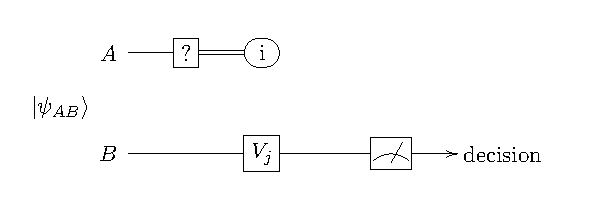
\includegraphics[scale=1.5]{onequbit.pdf}
%	\caption{A schematic representation of the setup for distinguishing
%		measurements using postselection.}
%	\label{postselection}
%\end{figure}






\begin{enumerate}
\item We prepare  the discriminator $\ket{\psi_{0}}$ on bipartite system.
\item We perform one of two quantum channels, either $\Phi_{\Id}$ or 
$\Phi_{U^\dagger}$,  on  the first part of the input state  $\ket{\psi_{0}}$, that means $\left( \Phi \otimes \Id\right)(\proj{\psi_0})$.
\item We measure the first part of the input state  $\ket{\psi_{0}}$ and 
receive an output label $i$.
\item  
Based on Holevo--Helstrom theorem, we perform a conditional binary 
measurement	$\PP_{V_j}$ and hence, we implement the quantum channel $\Phi_{V_j^\dagger}$ on the second part. 
\item To calculate the probability of correct discrimination, we include just those cases for which $i = j$.
\item We measure the second part of the input state  $\ket{\psi_{0}}$ and make a
decision based on received label $j$. If $i=j=0$, then we decide that  
$\PP_U$ occurs.  If $i=j=1$, we decide that 
$\PP_{\Id}$ occurs.
\end{enumerate}


The schematic representation of this setup is depicted in 
Fig.~\ref{fig:postsellection}.     

\begin{figure}[h!]
	\centering 
	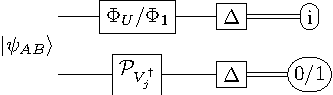
\includegraphics[scale=1.7]{pics/postselection} 
	
	\caption{ A schematic representation of the setup for distinguishing
		measurements using postselection. 
	}\label{fig:postsellection}
\end{figure}  

Due to the fact that the measurement result is nondeterministic, we are forced to consider the following circuits
in the postselection procedure
\begin{equation}
\begin{split}
(\Phi_{U^\dagger}, \Phi_{V_k^\dagger}, i, j) \\ 
(\Phi_{\Id}, \Phi_{V_k^\dagger}, i, j)
\end{split}
\end{equation}
where $k=\{0,1\}, i=\{0,1\}$ and $ j=\{0,1\}$. 
The optimal probability $p_{\text{succ}}(\PP_{U}, \PP_{\Id}) $ of correct discrimination between $\PP_{U} $ and $\PP_\Id$ is as follows
		\begin{equation}
		p_{\text{succ}}(\PP_{U}, \PP_{\Id})= \frac{\#(\Phi_{U^\dagger}, \Phi_{V_i^\dagger},i,0) + \#(\Phi_\Id, \Phi_{V_i^\dagger},i,1)}{\#(\Phi_{U^\dagger}, \Phi_{V_i^\dagger},i,j) + \#(\Phi_\Id, \Phi_{V_i^\dagger},i,j)}, 
		\end{equation}
where $i=\{0,1\}$ and $ j=\{0,1\}$. 

\end{scheme}


\begin{scheme}(By using controlled unitary)
	


\begin{enumerate}
\item We prepare the discriminator $\ket{\psi_{0}}$ on bipartite 
system. 
\item We perform one of two quantum channels, either $\Phi_{\Id}$ or
$\Phi_{U^\dagger}$,  on  the first part of the input state  $\ket{\psi_{0}}$, that means $\left(\Phi \otimes \Id\right)(\proj{\psi_0})$.
\item Based on Holevo--Helstrom theorem, we perform a conditional binary measurement $\PP_{V_j}$, and hence, we implement the direct sum of quantum channels $\Phi_{V_0^\dagger} \oplus \Phi_{V_1^\dagger}$. Observe that   $\Phi_{V_0^\dagger} \oplus \Phi_{V_1^\dagger} = \proj{0} \otimes \Phi_{V_0^\dagger}  + \proj{1} \otimes \Phi_{V_1^\dagger}.  $
\item We measure all systems in computational basis $\Delta$.
\item We make a decision based on received label $j$ on the second system. If $j=0$, then we
decide that $\PP_U$ occurs. Otherwise, we decide that $\PP_{\Id}$ occurs.
\end{enumerate}

The schematic representation of this setup is depicted in 
Fig.~\ref{fig:controlled}.     
\begin{figure}[h!]
	\centering 
	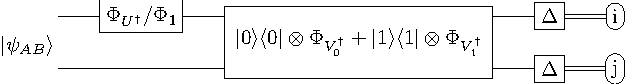
\includegraphics[scale=1.5]{pics/controlled_unitary} 
	
	\caption{ A schematic representation of the setup for distinguishing
		measurements using controlled unitary gate. 
	}\label{fig:controlled}
\end{figure} 


Here, we consider the following circuits
by using controlled unitary
\begin{equation}
\begin{split}
(\Phi_{U^\dagger}, \Phi_{V_0^\dagger} \oplus \Phi_{V_1^\dagger}, i, j) \\ 
(\Phi_{\Id},  \Phi_{V_0^\dagger} \oplus \Phi_{V_1^\dagger}, i, j)
\end{split}
\end{equation}
where $i=\{0,1\}$ and $ j=\{0,1\}$. 
Then, the optimal probability of correct discrimination between $\PP_{U} $ and $\PP_\Id$ is as follows.
\begin{equation}
p = \frac{\#(\Phi_{U^\dagger},\Phi_{V_0^\dagger} \oplus \Phi_{V_1^\dagger},i,0) + \#(\Phi_\Id,\Phi_{V_0^\dagger} \oplus \Phi_{V_1^\dagger},i,1) }{\#(\Phi_{U^\dagger},\Phi_{V_0^\dagger} \oplus \Phi_{V_1^\dagger},i,j) + \#(\Phi_\Id,\Phi_{V_0^\dagger} \oplus \Phi_{V_1^\dagger},i,j)}
\end{equation}
where $i=\{0,1\}$ and $ j=\{0,1\}$. 
\end{scheme}




\subsubsection{Mathematical preliminaries}


In this and the following sections we will denote complex Euclidean spaces $\mathbb{C}^d$ with $\XX, \mathcal{Y}$ etc. When needed the dimension of a space $\XX$ will be denoted $\dim(\XX)$. The set of matrices transforming vectors from $\XX$ to $\mathcal{Y}$ will be denoted $\mathrm{L}(\XX, \mathcal{Y})$.
 We will also need a linear mapping transforming $\mathrm{L}(\XX)$ into
$\mathrm{L}(\mathcal{Y})$, which will be denoted 
\begin{equation}
\Phi: \mathrm{L}(\XX) \rightarrow \mathrm{L}(\mathcal{Y}).
\end{equation} 
There
exists a bijection between introduced linear mappings $\Phi$ and set of matrices $\mathrm{L}(\mathcal{Y} \otimes \mathcal{X})$,  known as the Choi-
Jamio{\l}kowski isomorphism. 
For a given linear mapping $\Phi$ the corresponding  Choi operator $J(\Phi)$ is explicitly written as 
\begin{equation}
J(\Phi) \coloneqq \sum_{i,j=0}^{d- 1} \Phi(\ketbra{i}{j}) \otimes \ketbra{i}{j}. \end{equation}
Finally, we introduce a special subset of all mappings $\Phi$, called quantum channels, which are completely positive
and trace preserving (CPTP).
We will consider a special class of quantum channels, called unitary channels. A unitary channel
$\Phi_{U}$ is defined as $\Phi_U(\cdot) = U \cdot U^\dagger$ for  and unitary $U$. 



A general quantum
measurement, that is a positive operator valued measure (POVM) $\PP$ is a
collection of positive semidefinite operators $\{E_1, \ldots, E_m \}$ called
\emph{effects}, which sum up to identity, \ie $ \, \, \sum_{i=1}^m E_i = \1$. If
all the effects are rank-one projection operators, then such a measurement is
called a von Neumann measurement. Every von Neumann measurement can be
parameterized by a unitary matrix $U$ which the effects $\{\proj{u_0}, \ldots, \proj{u_{d-1}}\}$,
ale creating by taking $\ket{u_i}$ as  $i+1$-th column of the unitary matrix $U$. 
Hence, we will use the notation $\PP_{U}$. 
%
%
% The action of
%quantum measurement $\PP_{U}$ on some state $\rho \in \Omega_d$ can be
%seen as  a measure-and-prepare quantum channel as follows 
%$
%\PP_{U} : \rho \rightarrow \sum_{i=0}^{d-1} \bra{u_i} \rho \ket{u_i} \proj{i}.
%$ 

\subsubsection{Diamond norm and the task of discrimination between quantum operators}
This section defines a special norm on the space of linear mappings, known as 
the diamond norm, and establishes some of its properties. 
Next, we will explain the precise connection between the diamond
norm and the task of quantum operation discrimination. 


We define the diamond norm of a map $\Phi$ as 
\begin{equation}
\|\Phi\|_\diamond = \max_{\| \ket{\psi}\|_1=1} \| \left(\Phi \otimes \1\right) (\proj{\psi}) \|_1.
\end{equation}
The quantum state $\ket{\psi}$ which maximizes the diamond norm we will call as discriminator. 

The celebrated result by Helstrom~\cite{helstrom1976quantum} gives the optimal  probability of correct discrimination between two quantum measurements, $\PP$  and $\mathcal{Q}$, 
in terms of their distance with the use of the diamond norm
\begin{equation}
p_{\text{succ}}(\PP, \mathcal{Q}) =  \frac12 + \frac14 \| \PP - \mathcal{Q} \|_\diamond.
\end{equation}









\section{Illustrative Example}

Let us focus on single-qubit von Neumann measurements $\PP_\1$ and $\PP_U$.
Assume that the unitary matrix $U$ is of the form 
\begin{equation}
U = H 
\left(\begin{array}{cc}1&0\\0&e^{i \phi}\end{array}\right)  H^\dagger
\end{equation}
%\begin{equation}
%U = H \diag (1, \ee^{\ii \phi}) H^\dagger,
%\end{equation}
where $H$ is the Hadamard matrix of dimension two and $\phi \in [0, 2 \pi)$.

\subsubsection{Probability}\label{sec:example_probability}
\begin{theorem}
The optimal probability of correct discrimination between von Neumann
measurements $\PP_U$ and $\PP_{\Id}$ is given by
\begin{equation}
p_{\text{succ}}(\PP_{U}, \PP_{\Id}) = \frac{1}{2} + \frac{|1 - e^{i \phi}  |}{4} . 
\end{equation}
\end{theorem}







\subsubsection{Discriminator}\label{sec:example_discriminator}

\begin{proposition}\label{prop-discrim}
 The optimal input state has the form
\begin{equation}
\ket{\psi_{0}} = \frac{1}{\sqrt{2}} |\Id_2 \rangle \rangle.
\end{equation}
\end{proposition}



%

\subsubsection{Conditional binary measurement/Optimal measurement}\label{sec_example_final_measurement}



\begin{proposition}  
The  optimal measurement has the following form
\begin{equation}
\begin{split}
\mu(0) = \proj{0} \otimes V_0 \proj{0} V_0^\dagger +  \proj{1} \otimes V_1 
\proj{0} V_1^\dagger  \\ 
\mu(1) = \proj{0} \otimes V_0 \proj{1} V_0^\dagger +  \proj{1} \otimes V_1 
\proj{1} V_1^\dagger,
\end{split}
\end{equation}
where for each $\phi \in \mathbb{R}$ and  the unitaries $V_0$,  $V_1$ 
have the following form
\begin{equation}
V_0 = \left(\begin{array}{cc}i \sin\left( \frac{\pi - \phi}{4} \right)&-i 
\cos\left( \frac{\pi - \phi}{4} \right)\\ \cos\left( \frac{\pi - 
\phi}{4}\right)& \sin\left( \frac{\pi - \phi}{4} \right)\end{array}\right),
\end{equation}
\begin{equation}
V_1 = \left(\begin{array}{cc}-i \cos\left(\frac{\pi - \phi}{4}\right) &i 
\sin\left( \frac{\pi - \phi}{4}\right)\\\sin\left( \frac{\pi - \phi}{4} \right) 
&  \cos\left( \frac{\pi - \phi}{4} \right) \end{array}\right).
\end{equation}
\end{proposition}



 

\begin{thebibliography}{00}

\bibitem{preskill} Preskill, John. "Quantum Computing in the NISQ era and 
beyond." Quantum 2 (2018): 79.
\bibitem{michielsen2017benchmarking} Michielsen, Kristel, et al. "Benchmarking 
gate-based quantum computers." Computer Physics Communications 220 (2017): 
44-55.
\bibitem{zhukov2019quantum} Zhukov, A. A., et al. "Quantum communication 
protocols as a benchmark for programmable quantum computers." Quantum 
Information Processing 18.1 (2019): 1-23.
\bibitem{hamilton2018generative} Hamilton, Kathleen E., Eugene F. Dumitrescu, 
and Raphael C. Pooser. "Generative model benchmarks for superconducting 
qubits." Physical Review A 99.6 (2019): 062323.
\bibitem{benedetti2018generative} Benedetti, Marcello, et al. "A generative 
modeling approach for benchmarking and training shallow quantum circuits." npj 
Quantum Information 5.1 (2019): 1-9.
\bibitem{puchala2018strategies} Puchała, Zbigniew, et al. "Strategies for 
optimal single-shot discrimination of quantum measurements." Physical Review A 
98.4 (2018): 042103.
\bibitem{helstrom1976quantum} Helstrom, C. W. (1969). "Quantum detection and estimation theory." Journal of Statistical Physics, 1(2), 231-252.
\bibitem{watrous} Watrous, John (2018). The theory of quantum information. Cambridge university press.
\bibitem{nr} Lewandowska, Paulina and others. The web resource at \url{https://numericalshadow.org/}. Accessed on 2022-10-02. 
\bibitem{hausdorff} Hausdorff, Felix. "Der wertvorrat einer bilinearform." Mathematische Zeitschrift 3.1 (1919): 314-316.
\bibitem{toeplitz} Toeplitz, Otto. "Das algebraische Analogon zu einem Satze von Fejér." Mathematische Zeitschrift 2.1 (1918): 187-197.
\end{thebibliography}


\end{document}

%%
%% End of file `SoftwareX_article_template.tex'.

